\documentclass[12pt,a5paper,fleqn]{article}
\usepackage[utf8]{inputenc}
\usepackage{amssymb, amsmath, multicol}
\usepackage[russian]{babel}
\usepackage{graphicx}
\usepackage[shortcuts,cyremdash]{extdash}
\usepackage{wrapfig}
\usepackage{floatflt}
\usepackage{lipsum}
\usepackage{concmath}
\usepackage{euler}

\graphicspath{ {images/} }

\oddsidemargin=-17.9mm
\textwidth=133mm
\headheight=-35.4mm
\textheight=210mm
\parindent=0pt
\tolerance=100
\parskip=6pt
\pagestyle{empty}
\renewcommand{\tg}{\mathop{\mathrm{tg}}\nolimits}
\renewcommand{\ctg}{\mathop{\mathrm{ctg}}\nolimits}
\renewcommand{\arctan}{\mathop{\mathrm{arctg}}\nolimits}
\newcommand{\divisible}{\mathop{\raisebox{-2pt}{\vdots}}}
\renewcommand{\not}{\overline}

\RequirePackage{caption2}
\renewcommand\captionlabeldelim{}
\newcommand*{\hm}[1]{#1\nobreak\discretionary{}%
\newtheorem{Theorem}{Теорема}
{\hbox{$\mathsurround=0pt #1$}}{}}

\author{Старченко Иван}
\title{График по заданным данным}
\date{\today}

\begin{document}

\maketitle
\newpage

Таблица для данных:
\begin{center}
\includegraphics[width=10cm]{4}
\end{center}

\textit{График с анализом ниже}

\newpage

График с сглаживающей кривой первого порядка:
\begin{center}
\includegraphics[width=10cm]{1}
\end{center}

Анализ:
\begin{center}
\includegraphics[width=10cm]{5}
\end{center}



\newpage

График с сглаживающей кривой четвертого порядка:
\begin{center}
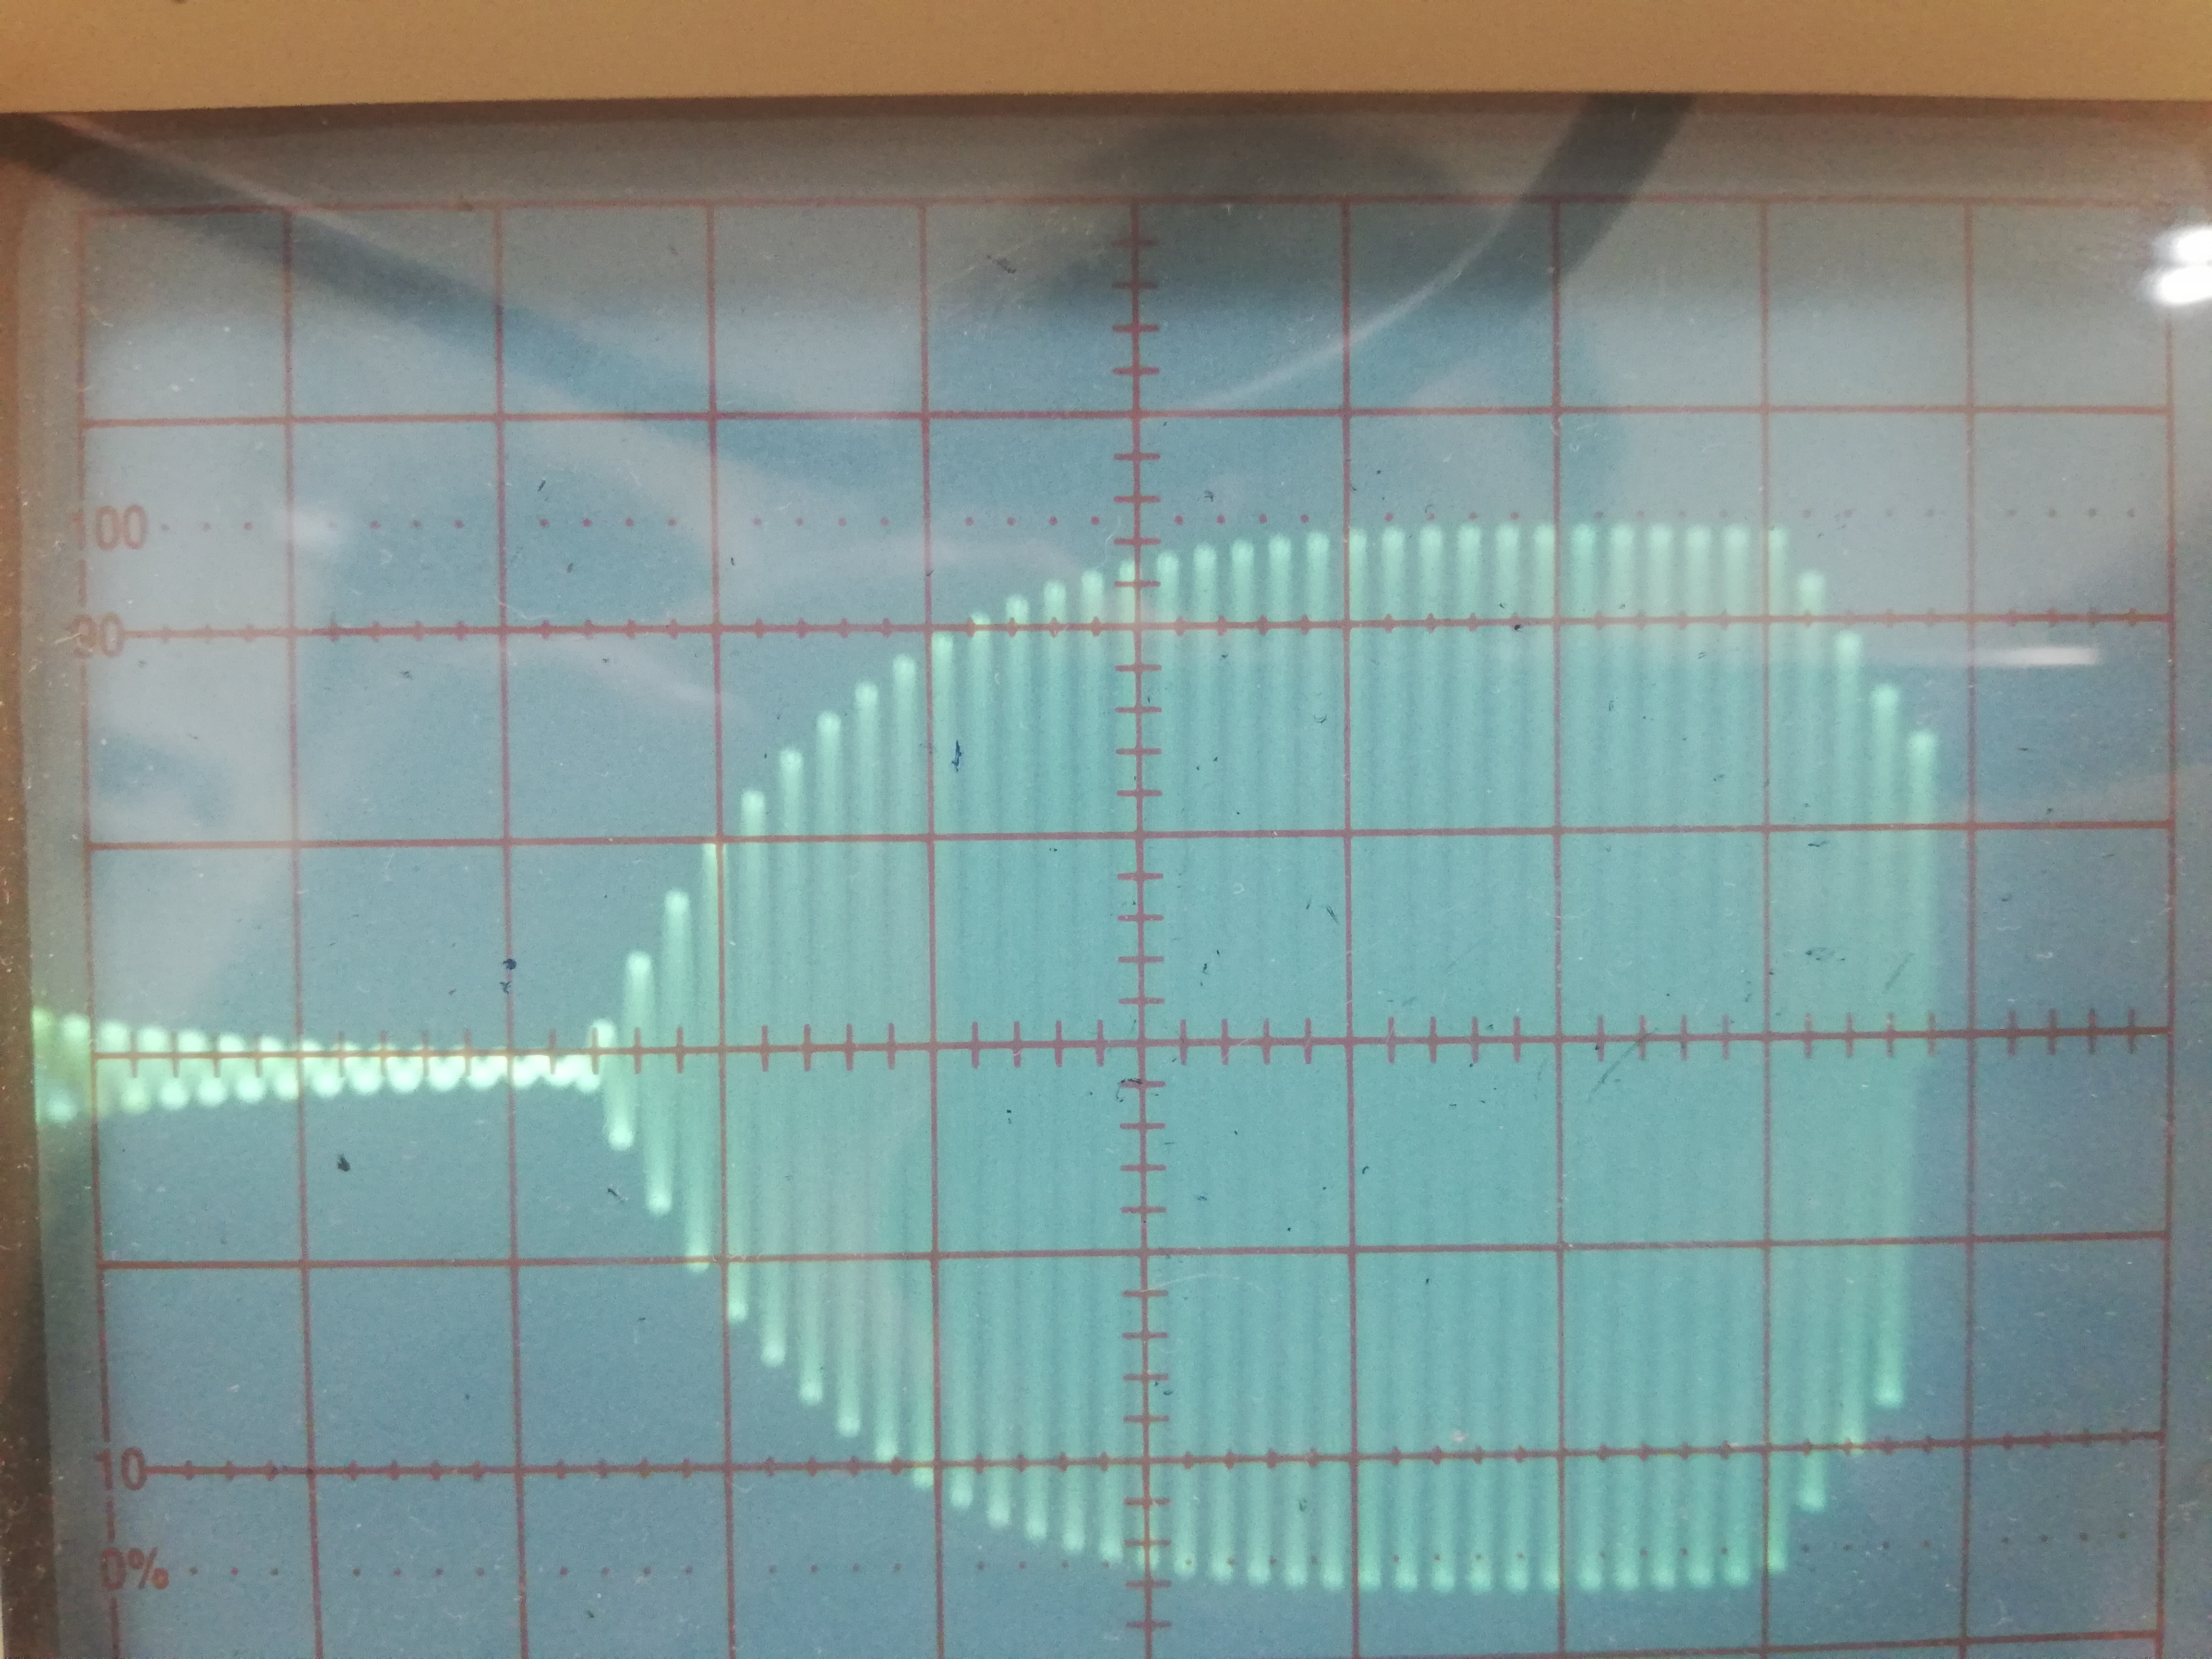
\includegraphics[width=10cm]{3}
\end{center}

Анализ:
\begin{center}
\includegraphics[width=10cm]{6}
\end{center}



\end{document}
